\section{Risultati}
\label{sec:risultati}
In questa sezione si valuteranno le performance dell'algoritmo.
Per condurre questa analisi si è innanzitutto creata una mappa riportata in figura
\ref{fig:dungeon} utilizzando il generatore di mappe 
\begin{figure}[!htb]
	\centering
	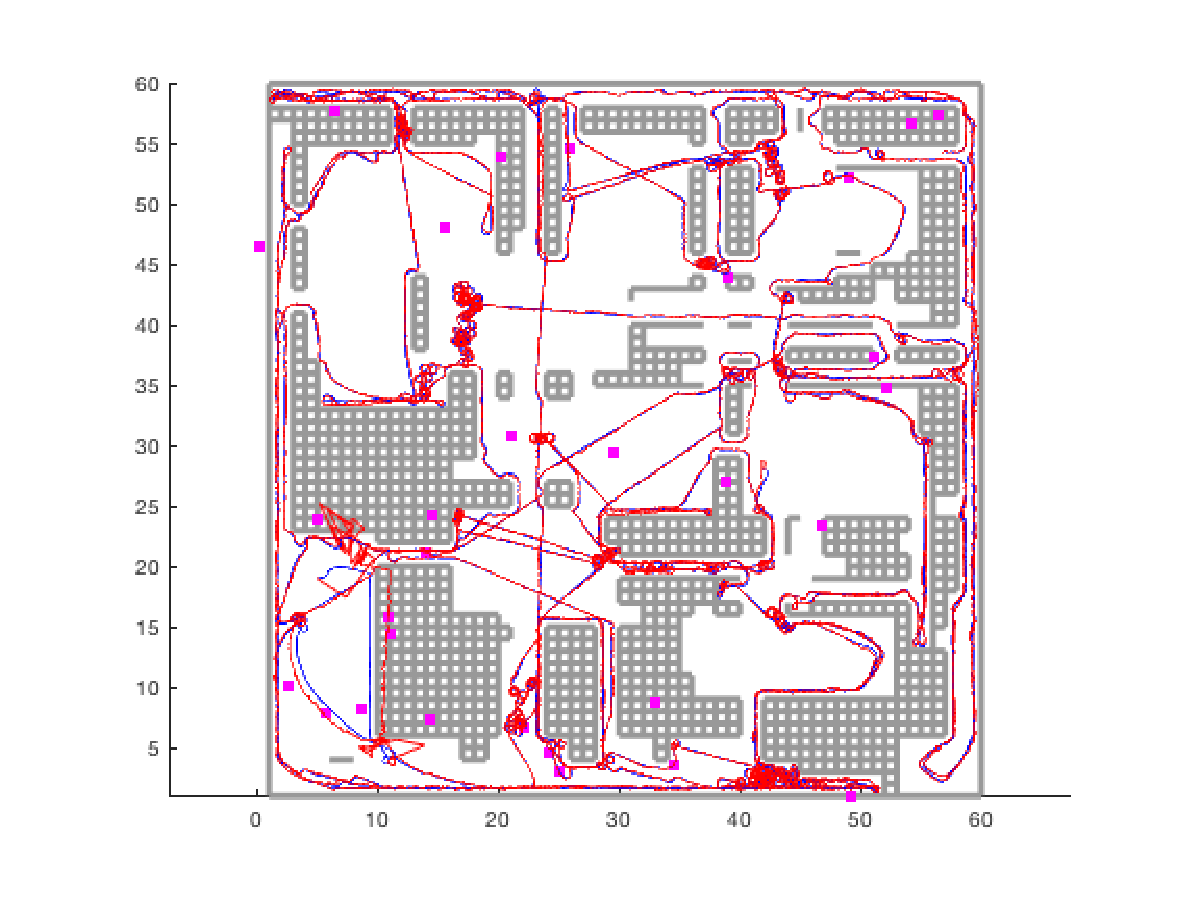
\includegraphics[width=\linewidth]{ParticleFilter}
	\caption{esempio di scenario procedurale $60\times60$}
\label{fig:dungeon}
\end{figure}
All'interno della mappa di figura \ref{fig:dungeon} sono riportate in blu le traiettorie vere
compiute dai robot mentre in rosso le traiettorie stimate. Le traiettorie riportate sono quelle
ottenute compiendo una simualzione di 1800 secondi e tramite l'utilizzo di 3 robot che 
contemporaneamente la esplorano. La scelta di tale numero di robot e tempo di simulazione 
è stata compiuta per rispondere a 2 quesiti principali: efficienza energetica e percentuale di
mappa esplorata. In figura \ref{fig:TotalDistance} si può condurre il primo tipo di studio 
considerando che il percorrere una distanza maggiore comporta un maggiore dispendio
energetico mentre in figura \ref{fig:ExploredMap} si può notare come spesso l'adottare un 
numero maggiore di robot porti ad un'esplorazione più veloce. Osservando entrambi i grafici 
si può evidenziare che l'adozione di 4 robot rispetto a 3 non comporti grossi benefici in termini di
esplorazione percentuale della mappa, ricade allora sul numero di 3 robot la nostra scelta in
quanto come evidanziato dal grafico \ref{fig:TotalDistance} questo comporta un dispendio energetico 
minore.Mentre il tempo totale di 1800 secondi è stato scelto in quanto a tale lunghezza della 
simulazione si ottiene un valore ragionevole di mappa esplorata $70\%$.
La percentuale di mappa esplorata è stata ottenuta considerando il numero totale di 
celle libere realmente a disposizione rispetto al numero di celle viste dal robot, come riportato
nella equazione \ref{eq:FracMap}.

\begin{equation}
Mappa Esplorata = \frac{Celle Libere}{Celle Visitate} \cdot 100 \%
\label{eq:FracMap}
\end{equation}

\begin{figure}[!htb]
	\centering
	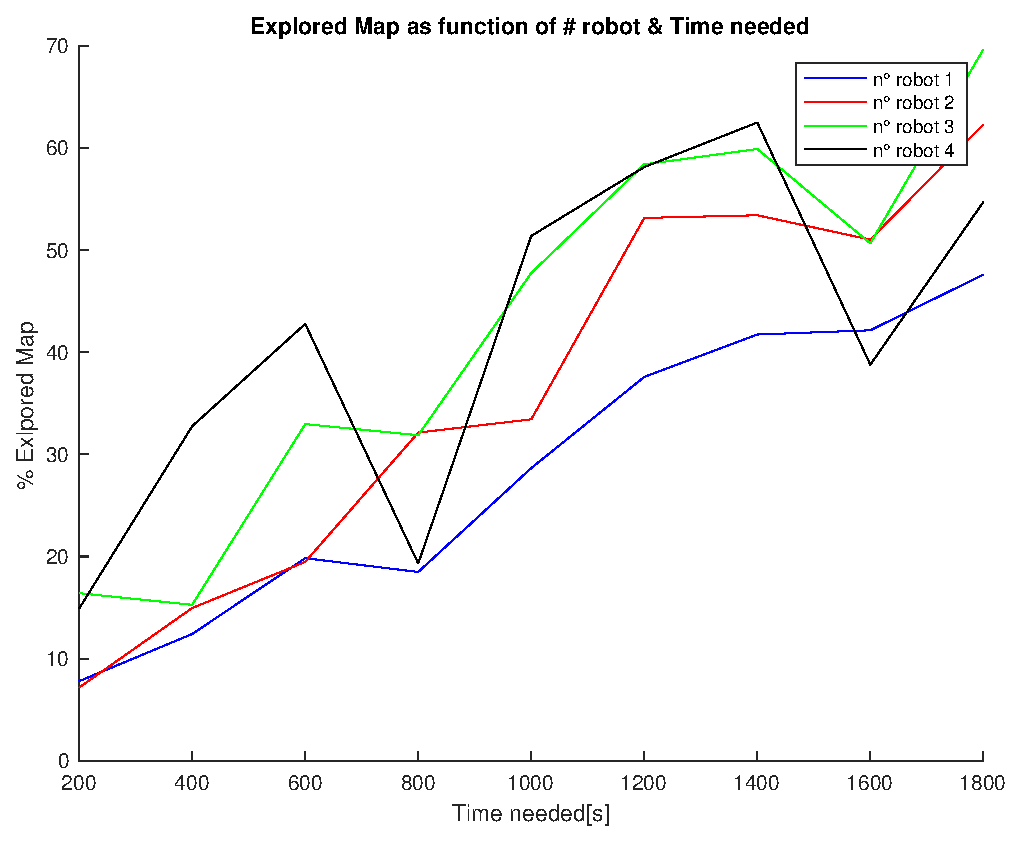
\includegraphics[width=\linewidth]{ExploredMap}
	\caption{Percentuale di mappa esplorata per \# robot e tempo di simulazione}
\label{fig:ExploredMap}
\end{figure}

\begin{figure}[!htb]
	\centering
	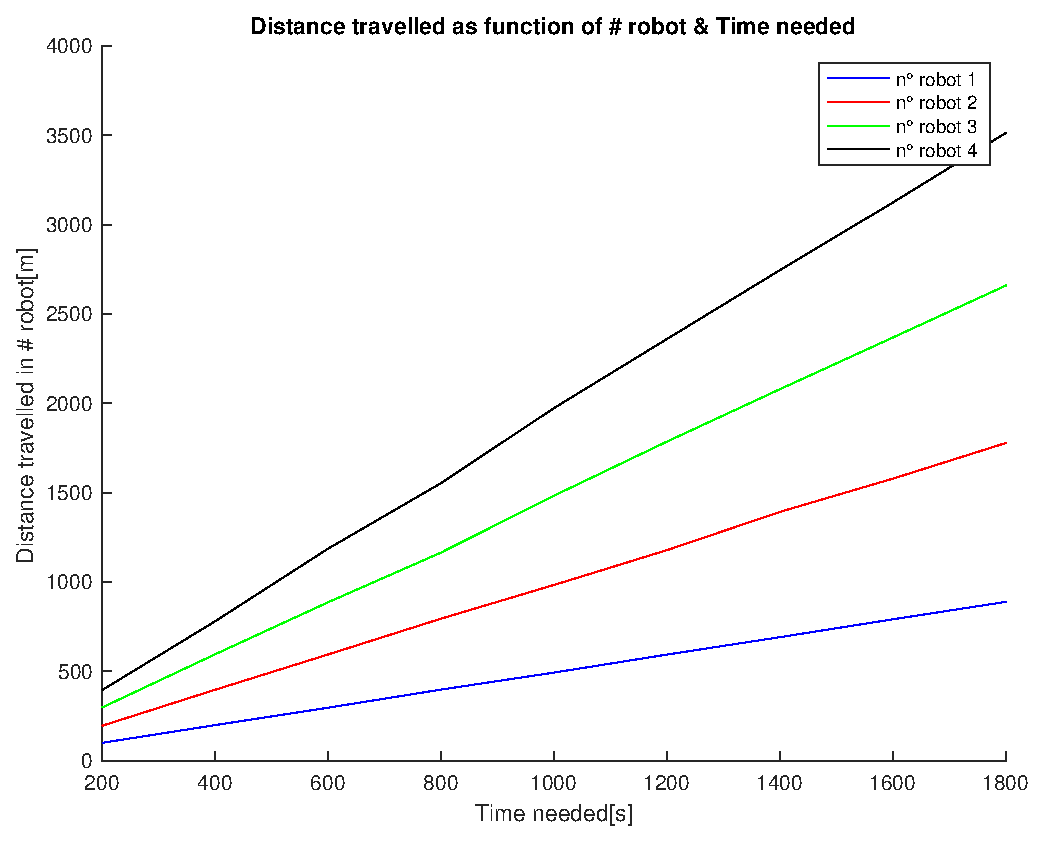
\includegraphics[width=\linewidth]{TotalDistance}
	\caption{Totale della distanza percorsa per \# robot e tempo di simulazione}
\label{fig:TotalDistance}
\end{figure}
\begin{table}[htb]
	\centering
	\caption{Risultati ottenuti}
	\label{tab:optimalresults}
	\begin{tabular}{lcS[table-format=3.2]}
	\toprule
	\multicolumn{3}{c}{dimensioni}\\
	\midrule
      numero ottimo di robot  & [ \# ] & 3\\
      tempo ottimo di simulazione     & [\si{\second}] & 1800\\
     \bottomrule
\end{tabular}
\end{table}

Scelto il numero ottimo di robot e tempo di simulazione \ref{tab:optimalresults} si può ottenere
le mappe fornite da questi. In figura \ref{fig:IdealMap} viene riportata la mappa fornita dai 3 robot
in caso di esplorazione ideale dove drift da parte dei sistemi robotici non sono considerati. In figura
\ref{fig:RealMap} viene riportata la mappa fornita in caso di presenza di drift nel sistema e necessità
di correzione dello stato dei robot tramite il particle filter. 
\begin{figure}[!htb]
	\centering
	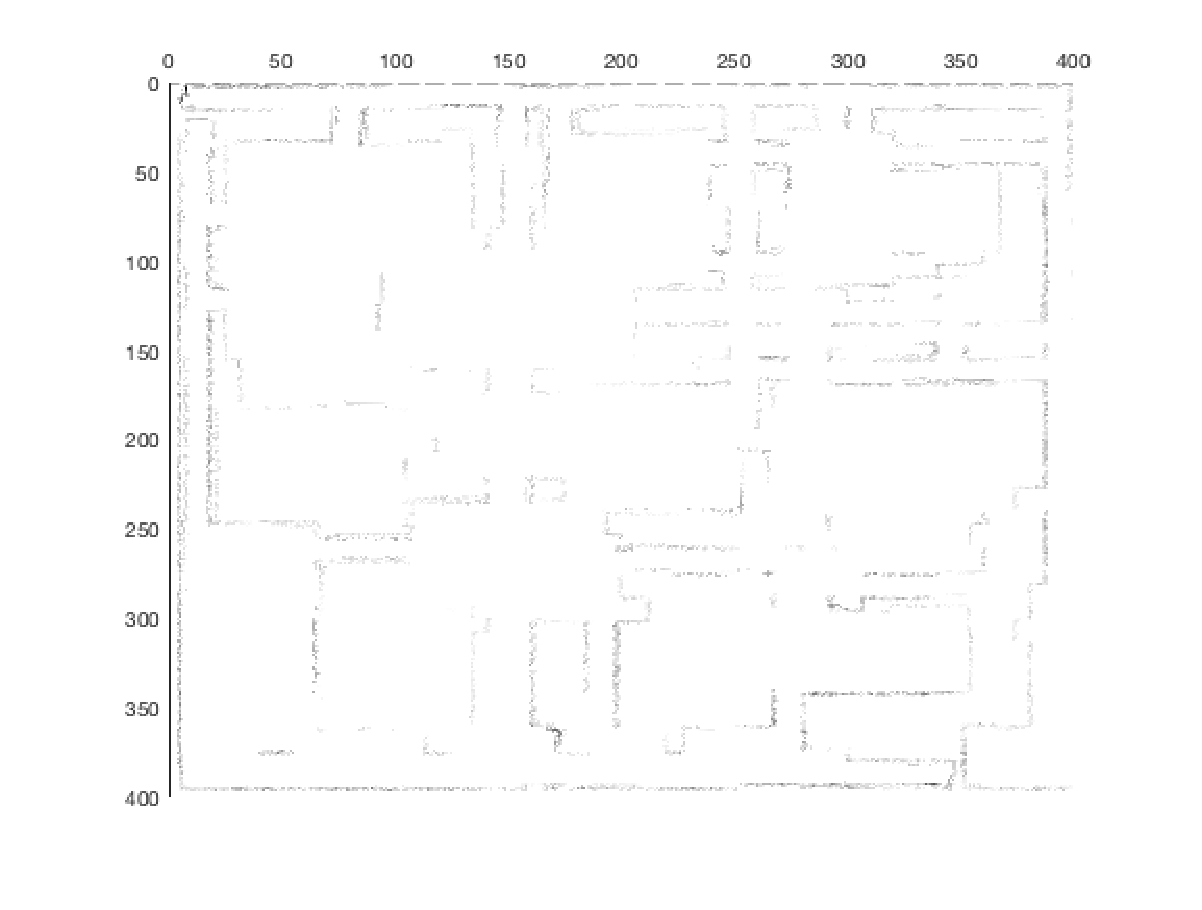
\includegraphics[width=\linewidth]{IdealMap}
	\caption{Raffigurazione della Mappa Ideale fornita dai robot con la data risoluzione di 0.15 [m]}
\label{fig:IdealMap}
\end{figure}

\begin{figure}[!htb]
	\centering
	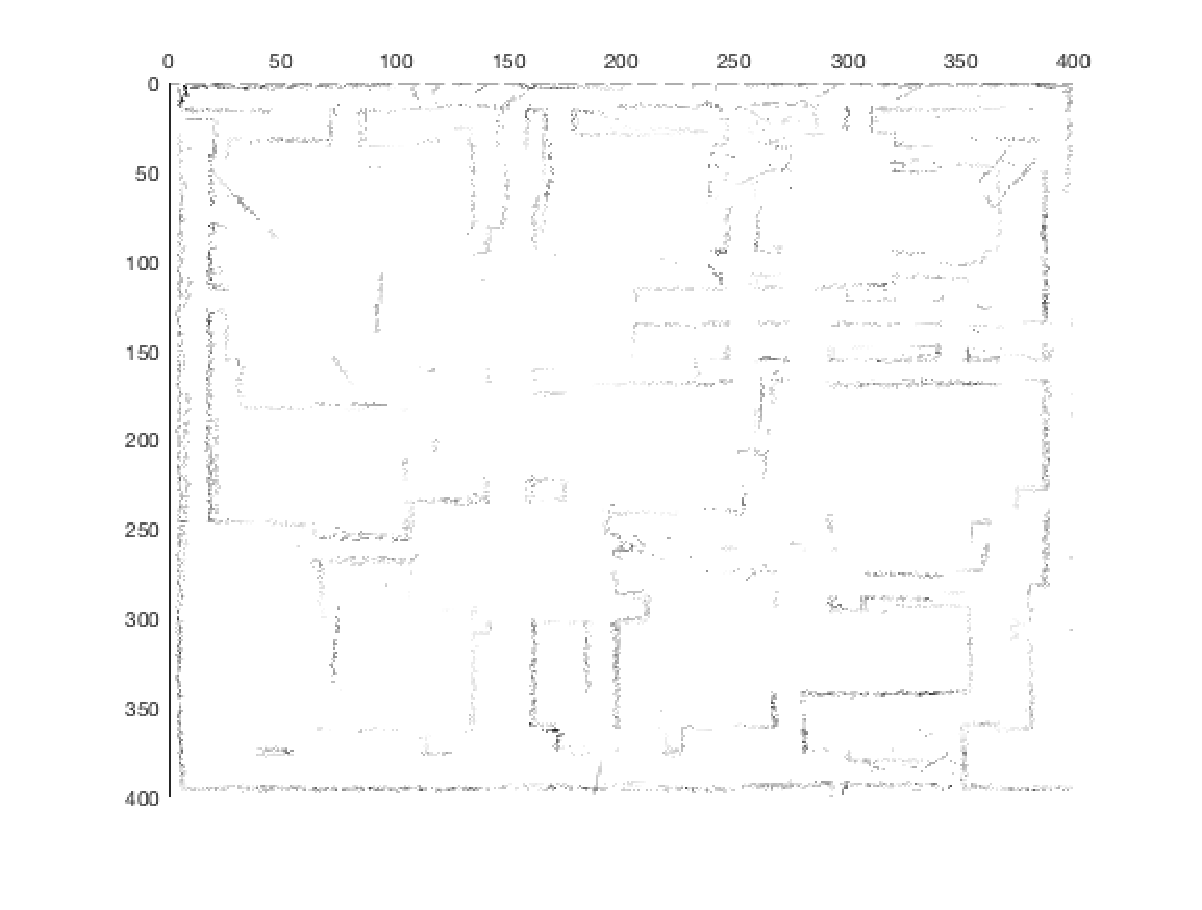
\includegraphics[width=\linewidth]{RealMap}
	\caption{Raffigurazione della Mappa Reale fornita dai robot con la data risoluzione di 0.15 [m] }
\label{fig:RealMap}
\end{figure}
